\documentclass[a4paper, 12pt]{article}
\usepackage[utf8x]{inputenc}
\usepackage{cmap}
\usepackage[english, russian]{babel}
\usepackage{indentfirst}
\usepackage[left=20mm, top=20mm, right=20mm, bottom=20mm]{geometry}
\usepackage{tikz}
\usepackage{float}
\usepackage{amsmath, amsfonts, amssymb}
\usepackage{graphicx}
\usepackage{fancybox, fancyhdr}
\usepackage{hyperref}
\usepackage{listings}
\usepackage{caption}
\usepackage{subcaption}
\usepackage{xcolor}
\usepackage{paralist}
\pagestyle{fancy}
\fancyhf{}
\fancyhead[L]{Лабораторная работа №2}
\fancyhead[R]{Линейные системы автоматического управления}
\fancyfoot[C]{\thepage}
\graphicspath{{images/}}
\usetikzlibrary{patterns}
\definecolor{LightGray}{gray}{0.95}
\definecolor{LightGray2}{gray}{0.7}
\hypersetup{
    colorlinks=true,
    linkcolor=blue,
    filecolor=magenta,
    urlcolor=cyan,
    pdftitle={contents setup},
    pdfpagemode=FullScreen,
}
\setlength{\parskip}{1.5mm}
\setlength{\headheight}{15pt}
\setlength{\footskip}{15pt}
\allowdisplaybreaks

\begin{document}
    \begin{titlepage}

        \begin{center}
        
\includegraphics[width=0.3\textwidth]{itmo.png} % requires itmo.png in /images folder
        \vfill
        
        Федеральное государственное автономное образовательное учреждение высшего образования
        «Национальный Исследовательский Университет ИТМО»\\
        
        \vfill
        {\large\bf ЛАБОРАТОРНАЯ РАБОТА №2}\\
        {\large\bf ПРЕДМЕТ «ЛИНЕЙНЫЕ СИСТЕМЫ АВТОМАТИЧЕСКОГО УПРАВЛЕНИЯ»}\\
        {\large\bf ТЕМА «КАНОНИЧЕСКИЕ ФОРМЫ ПРЕДСТАВЛЕНИЯ ДИНАМИЧЕСКИХ СИСТЕМ»}\\
        Вариант 4
        \vfill

        \begin{flushright}
            \begin{minipage}{.45\textwidth}
            {
                \hbox{Преподаватель: Золотаревич В. П.}
                \hbox{Студент: Румянцев А. А.}
                \hbox{Поток: ЛСАУ R22 бак 4.1.1}
                \hbox{}
                \hbox{Факультет: СУиР}
                \hbox{Группа: R3341}
            }
            \end{minipage}
        \end{flushright}
        
        \vfill
                
        Санкт-Петербург\\
        2024
        \end{center}
    \end{titlepage}
    
    \tableofcontents

    \newpage
    \section{Цель работы}
    Ознакомление с методами взаимного перехода между моделями \\
    вход-выход и вход-состояние-выход, а также с каноническими формами представления
    моделей вход-состояние-выход.


    \section{Задание 1}
    \subsection{Условие}
    \textit{Переход от модели вход-выход к модели вход-состояние-выход.}
    \begin{compactitem}
        \item Построить математические модели вход-состояние-выход
        в канонической управляемой и канонической
        наблюдаемой формах. Определить передаточную функцию системы. Дано:
        $$n=3,\ \ a_0=8,\ \ a_1=6,\ \ a_2=2,\ \ b_0=12,\ \ b_1=1,\ \ b_2=10$$
        \item Используя блоки ``Transfer Fcn'' и ``State-Space'' пакета SIMULINK,
        осуществить моделирование моделей вход-выход, вход-состояние-выход в канонической
        управляемой форме и вход-состояние-выход в канонической наблюдаемой форме при
        ступенчатом единичном входном воздействии и нулевых начальных условиях. Схема
        моделирования иллюстрируется рис. \ref{fig:scheme1}, где блок с именем ``Transfer Fcn'' задает модель
        вход-выход в форме передаточной функции, блок ``State-Space'' -- модель вход-
        состояние-выход в канонической управляемой форме, а блок ``State-Space1'' -- модель
        вход-состояние-выход в канонической наблюдаемой форме.
        \begin{figure}[H]
            \centering
            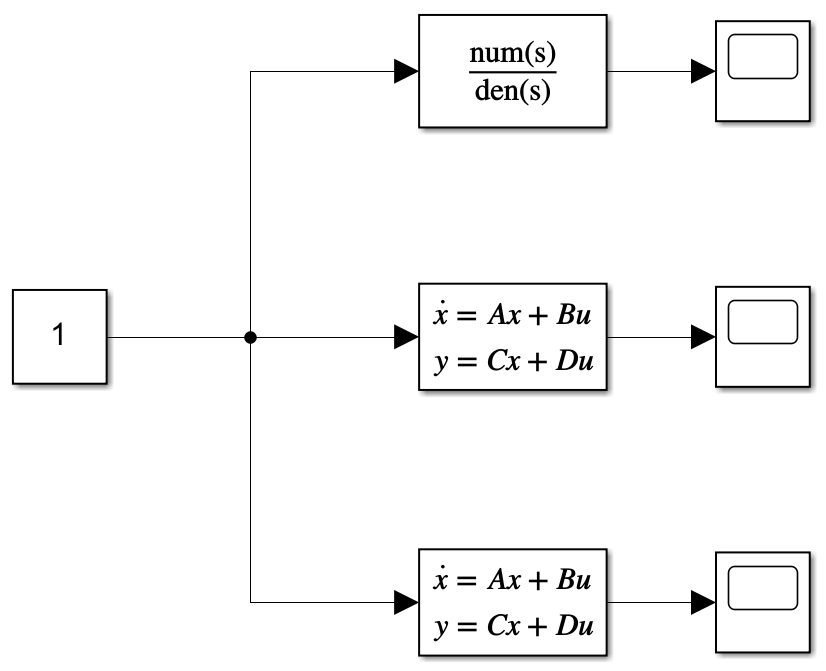
\includegraphics[scale=0.5]{scheme1.png}
            \captionsetup{skip=0pt}
            \caption{Схема эксперимента}
            \label{fig:scheme1}
        \end{figure}
    \end{compactitem}
    

    \subsection{Выполнение}
    Составим уравнение
    $$y^{(3)}+2y^{(2)}+6y^{(1)}+8y=10u^{(2)}+u^{(1)}+12u$$
    Сделаем замену $p=d/dt$
    $$p^3y+2p^2y+6py+8y=10p^2u+pu+12u$$
    Вынесем за скобки общие множители $y$ и $u$
    $$y(p^3+2p^2+6p+8)=u(10p^2+p+12)$$
    Найдем передаточную функцию
    $$W(p)=\dfrac{y}{u}=\dfrac{10p^2+p+12}{p^3+2p^2+6p+8}$$
    Разложим на систему уравнений с передаточной функцией. Переменная $z$ служит для связи между входом $u$ и выходом $y$
    $$
    \begin{cases}
        (p^3+2p^2+6p+8)z=u\\
        (10p^2+p+12)z=y
    \end{cases}
    $$
    Каноническая управляемая форма будет иметь вид
    $$
    A=
    \begin{bmatrix}
        0 & 1 & 0\\
        0 & 0 & 1\\
        -8 & -6 & -2
    \end{bmatrix},\ \
    B=
    \begin{bmatrix}
        0\\
        0\\
        1
    \end{bmatrix},\ \
    C=
    \begin{bmatrix}
        12 & 1 & 10
    \end{bmatrix}
    $$
    Записывается в виде системы как
    $$
    \begin{cases}
        \dot{x}_1=x_2\\
        \dot{x}_2=x_3\\
        \dot{x}_3=-8x_1-6x_2-2x_3+u\\
        y=12x_1+x_2+10x_3
    \end{cases}
    $$
    Каноническая наблюдаемая форма будет иметь вид
    $$
    A=
    \begin{bmatrix}
        0 & 0 & -8\\
        1 & 0 & -6\\
        0 & 1 & -2
    \end{bmatrix},\ \
    B=
    \begin{bmatrix}
        12\\
        1\\
        10
    \end{bmatrix},\ \
    C=
    \begin{bmatrix}
        0 & 0 & 1
    \end{bmatrix}
    $$
    Записывается в виде системы как
    $$
    \begin{cases}
        \dot{x}_1=-8x_3+12u\\
        \dot{x}_2=x_1-6x_3+u\\
        \dot{x}_3=x_2-2x_3+10u\\
        y=x_3
    \end{cases}
    $$
    Схема моделирования представлена на рис. \ref{fig:scheme1}. Параметры в SIMULINK представлены на рис. \ref{fig:windows1}. Выведем графики.
    \begin{figure}[H]
        \centering
        \begin{subfigure}{0.3\textwidth}
            \centering
            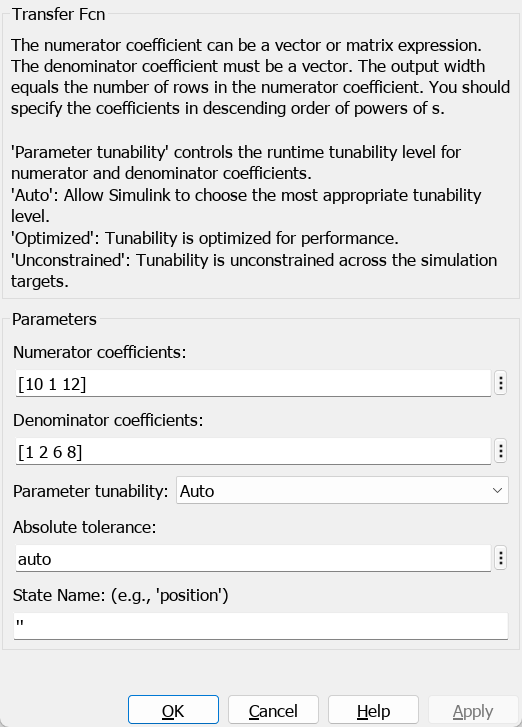
\includegraphics[width=\linewidth]{W_p_1_window.png}
            \caption{Параметры SIMULINK для передаточной функции $W(p)$}
            \label{fig:wp1w}
        \end{subfigure}
        \begin{subfigure}{0.3\textwidth}
            \centering
            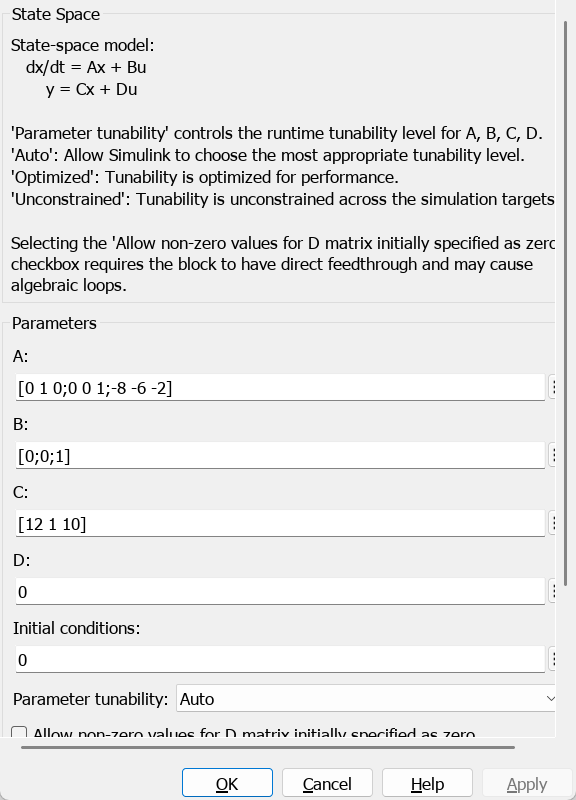
\includegraphics[width=\linewidth]{canonical_controlled_form_1_window.png}
            \caption{Параметры SIMULINK для канонической управляемой формы}
            \label{fig:ccf1w}
        \end{subfigure}
        \begin{subfigure}{0.3\textwidth}
            \centering
            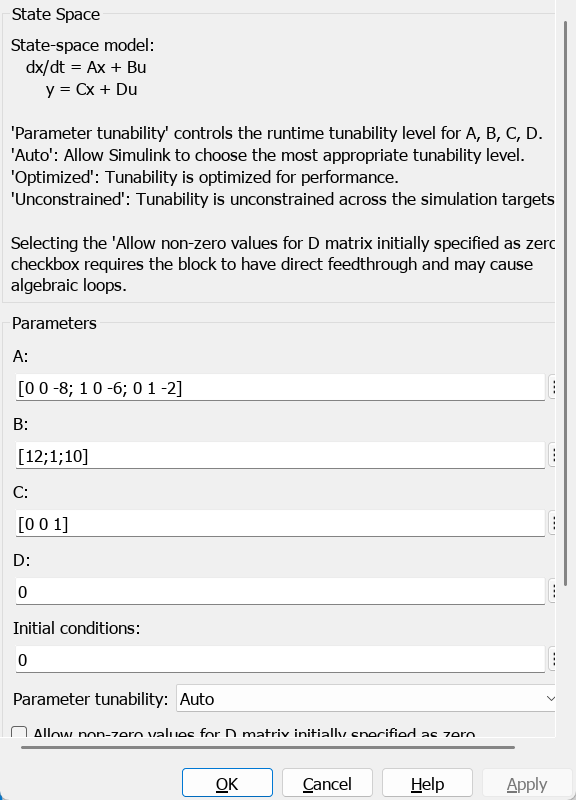
\includegraphics[width=\linewidth]{canonical_observable_form_1_window.png}
            \caption{Параметры SIMULINK для канонической наблюдаемой формы}
            \label{fig:cof1w}
        \end{subfigure}
        \caption{Параметры SIMULINK для ``Transfer Fcn'' и ``State-Space''}
        \label{fig:windows1}
    \end{figure}
    \begin{figure}[H]
        \centering
        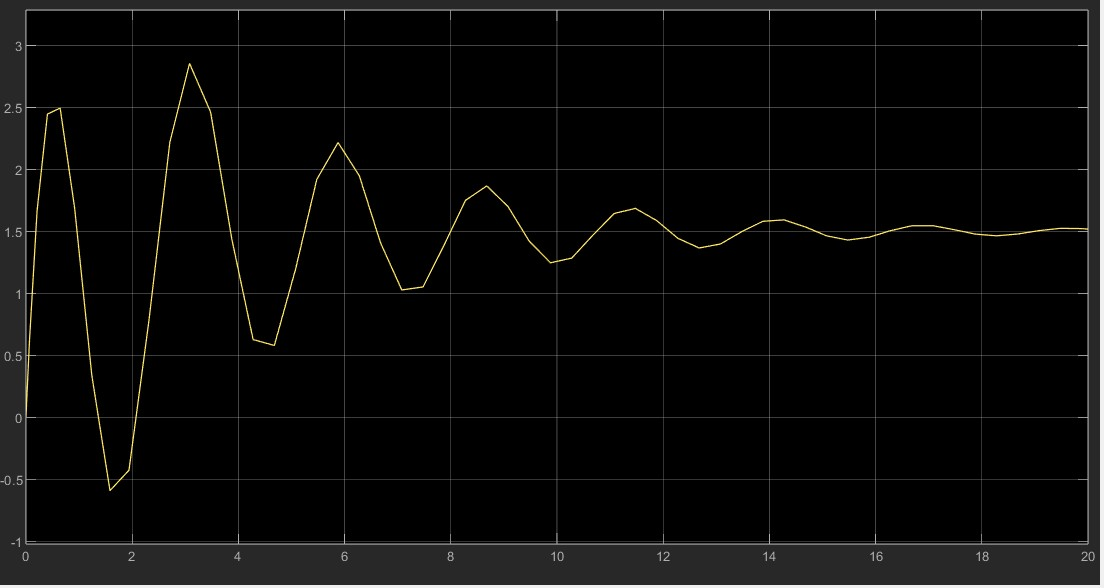
\includegraphics[scale=0.3]{W_p_1.jpg}
        \captionsetup{skip=0pt}
        \caption{График передаточной функции $W(p)$}
        \label{fig:wp1}
    \end{figure}
    \begin{figure}[H]
        \centering
        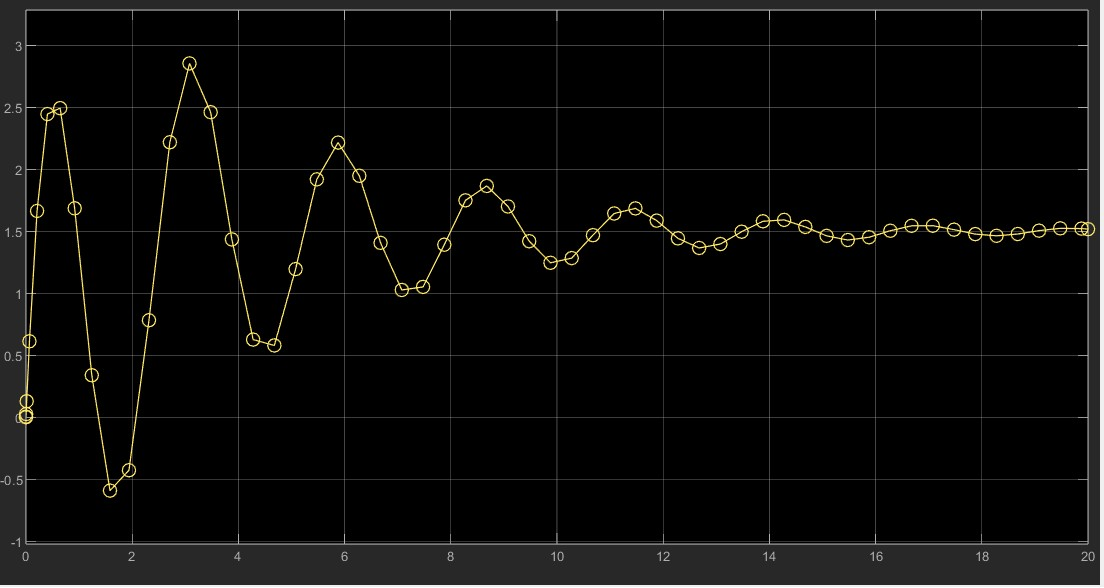
\includegraphics[scale=0.3]{canonical_controlled_form_1.jpg}
        \captionsetup{skip=0pt}
        \caption{График канонической управляемой формы}
        \label{fig:ccf1}
    \end{figure}
    \begin{figure}[H]
        \centering
        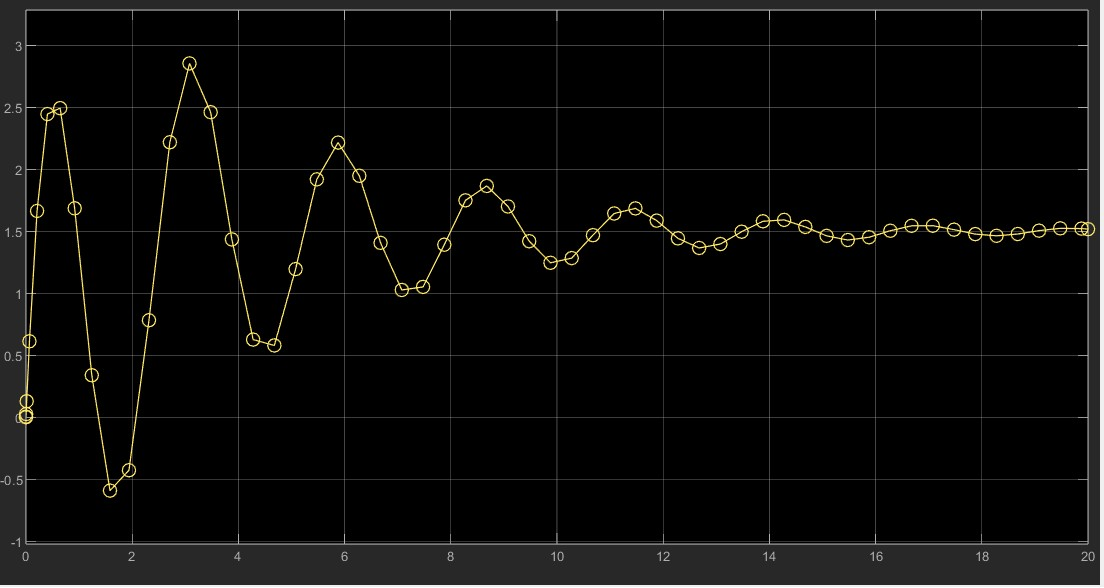
\includegraphics[scale=0.3]{canonical_observable_form_1.jpg}
        \captionsetup{skip=0pt}
        \caption{График канонической наблюдаемой формы}
        \label{fig:cof1}
    \end{figure}


    \section{Задание 2}
    \subsection{Условие}
    \textit{Переход от модели вход-состояние-выход к модели вход-выход.}
    \begin{compactitem}
    \item Осуществить расчет передаточной функции системы, а также канонических моделей вход-состояние-выход. Дано:
    $$n=2,\ \ A=
    \begin{bmatrix}
        0.5 & 1\\
        -15 & -3
    \end{bmatrix},\ \
    B=
    \begin{bmatrix}
        0\\
        1
    \end{bmatrix},\ \
    C=
    \begin{bmatrix}
        5 & 1
    \end{bmatrix}$$
    \item Используя блоки ``Transfer Fcn'' и ``State-Space'' пакета SIMULINK,
    осуществить моделирование исходной модели и полученных моделей вход-выход,
    вход-состояние-выход в канонической управляемой форме и вход-состояние-выход
    в канонической наблюдаемой форме, при ступенчатом единичном входном воздействии
    и нулевых начальных условиях
    \item Рассчитать матрицы преобразования исходной модели к каноническим формам.
    \end{compactitem}


    \subsection{Выполнение}
    Найдем передаточную функцию по формуле
    $$W(p)=C(pI-A)^{-1}B$$
    Проведем расчеты
    $$pI-A=
    p
    \begin{bmatrix}
        1 & 0\\
        0 & 1
    \end{bmatrix}
    -
    \begin{bmatrix}
        0.5 & 1\\
        -15 & -3
    \end{bmatrix}
    =
    \begin{bmatrix}
        \frac{2p-1}{2} & -1\\
        15 & p+3
    \end{bmatrix}$$
    $$(pI-A)^{-1}=
    \begin{bmatrix}
        \frac{2p-1}{2} & -1\\
        15 & p+3
    \end{bmatrix}^{-1}=
    \dfrac{1}{2p^2+5p+27}
    \begin{bmatrix}
        2p+6 & 2\\
        -30 & 2p-1
    \end{bmatrix}$$
    $$C(pI-A)^{-1}=\begin{bmatrix}
        5 & 1
    \end{bmatrix}
    \dfrac{1}{2p^2+5p+27}
    \begin{bmatrix}
        2p+6 & 2\\
        -30 & 2p-1
    \end{bmatrix}=
    \dfrac{1}{2p^2+5p+27}
    \begin{bmatrix}
        10p & 2p+9
    \end{bmatrix}$$
    $$C(pI-A)^{-1}B=\dfrac{1}{2p^2+5p+27}
    \begin{bmatrix}
        10p & 2p+9
    \end{bmatrix}
    \begin{bmatrix}
        0\\
        1
    \end{bmatrix}=
    \dfrac{2p+9}{2p^2+5p+27}
    $$
    Таким образом,
    $$W(p)=\dfrac{2p+9}{2p^2+5p+27}=\dfrac{p+4.5}{p^2+2.5p+13.5}$$
    Разложение на систему уравнений имеет вид
    $$
    \begin{cases}
        (p^2+2.5p+13.5)z=u\\
        (p+4.5)z=y
    \end{cases}
    $$
    Каноническая управляемая форма будет иметь вид
    $$
    A=
    \begin{bmatrix}
        0 & 1\\
        -13.5 & -2.5
    \end{bmatrix},\ \
    B=
    \begin{bmatrix}
        0\\
        1
    \end{bmatrix},\ \
    C=
    \begin{bmatrix}
        4.5 & 1
    \end{bmatrix}
    $$
    Записывается в виде системы как
    $$
    \begin{cases}
        \dot{x}_1=x_2\\
        \dot{x}_2=-13.5x_1-2.5x_2+u\\
        y=4.5x_1+x_2
    \end{cases}
    $$
    Каноническая наблюдаемая форма будет иметь вид
    $$
    A=
    \begin{bmatrix}
        0 & -13.5\\
        1 & -2.5
    \end{bmatrix},\ \
    B=
    \begin{bmatrix}
        4.5\\
        1
    \end{bmatrix},\ \
    C=
    \begin{bmatrix}
        0 & 1
    \end{bmatrix}
    $$
    Записывается в виде системы как
    $$
    \begin{cases}
        \dot{x}_1=-13.5x_2+4.5u\\
        \dot{x}_2=x_1-2.5x_2+u\\
        y=x_2
    \end{cases}
    $$
    Схема моделирования представлена на рис. \ref{fig:scheme1}. Параметры в SIMULINK представлены на рис. \ref{fig:windows2}. Выведем графики.
    \begin{figure}[H]
        \centering
        \begin{subfigure}{0.3\textwidth}
            \centering
            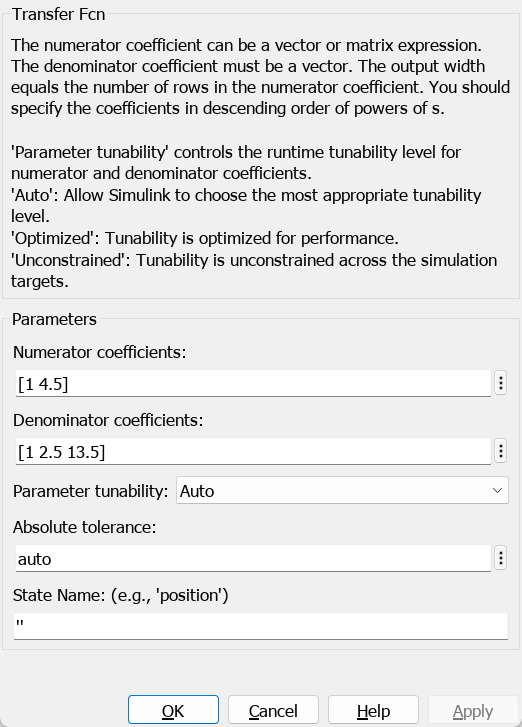
\includegraphics[width=\linewidth]{W_p_2_window.png}
            \caption{Параметры SIMULINK для передаточной функции $W(p)$}
            \label{fig:wp2w}
        \end{subfigure}
        \begin{subfigure}{0.3\textwidth}
            \centering
            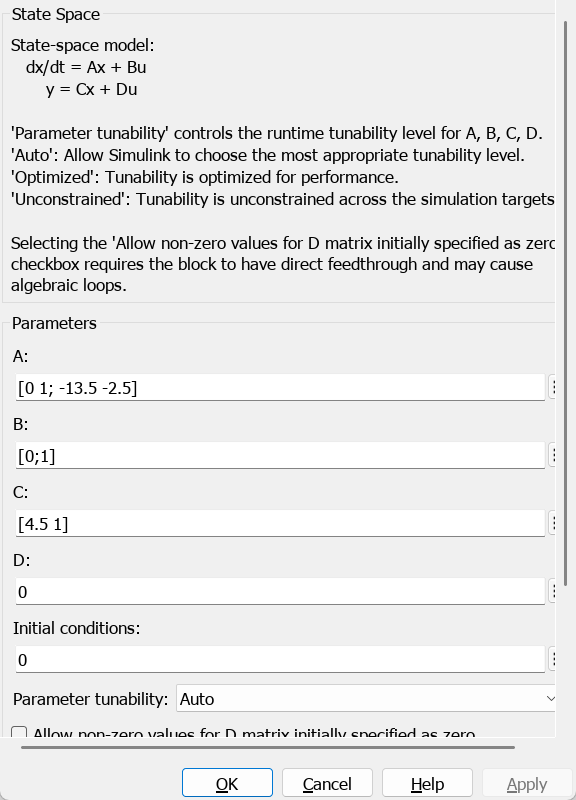
\includegraphics[width=\linewidth]{canonical_controlled_form_2_window.png}
            \caption{Параметры SIMULINK для канонической управляемой формы}
            \label{fig:ccf2w}
        \end{subfigure}
        \begin{subfigure}{0.3\textwidth}
            \centering
            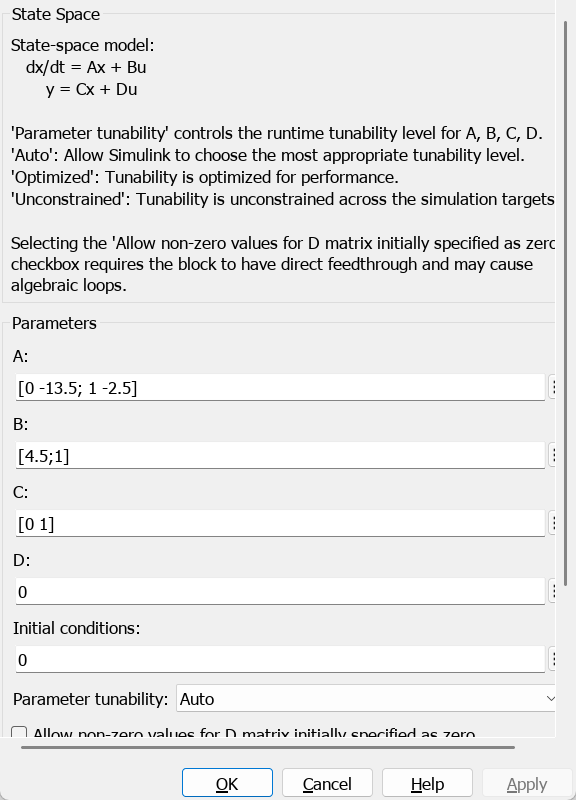
\includegraphics[width=\linewidth]{canonical_observable_form_2_window.png}
            \caption{Параметры SIMULINK для канонической наблюдаемой формы}
            \label{fig:cof2w}
        \end{subfigure}
        \caption{Параметры SIMULINK для ``Transfer Fcn'' и ``State-Space''}
        \label{fig:windows2}
    \end{figure}
    \begin{figure}[H]
        \centering
        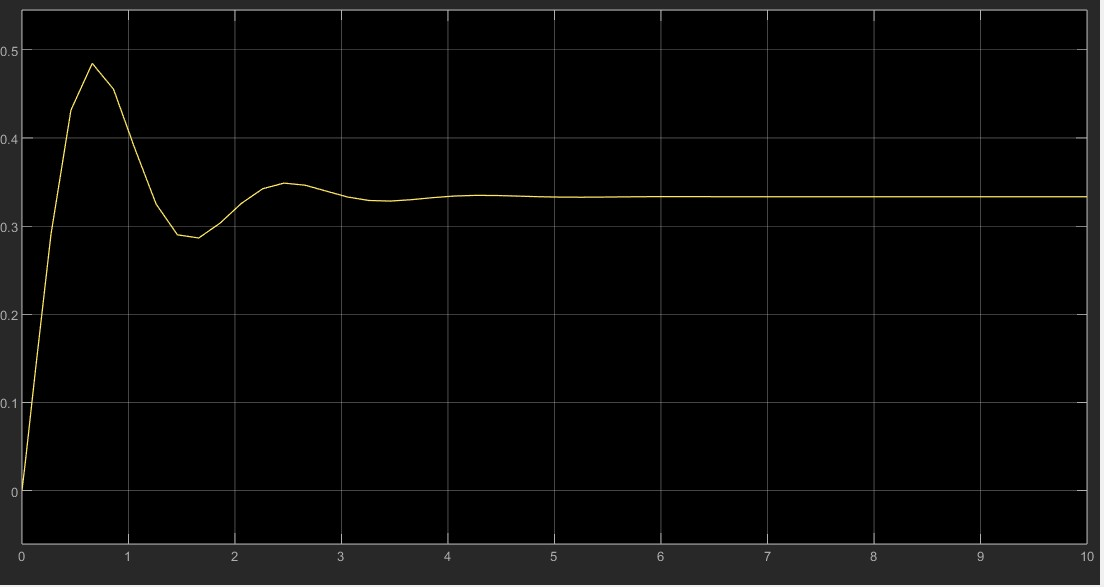
\includegraphics[scale=0.3]{W_p_2.jpg}
        \captionsetup{skip=0pt}
        \caption{График передаточной функции $W(p)$}
        \label{fig:wp2}
    \end{figure}
    \begin{figure}[H]
        \centering
        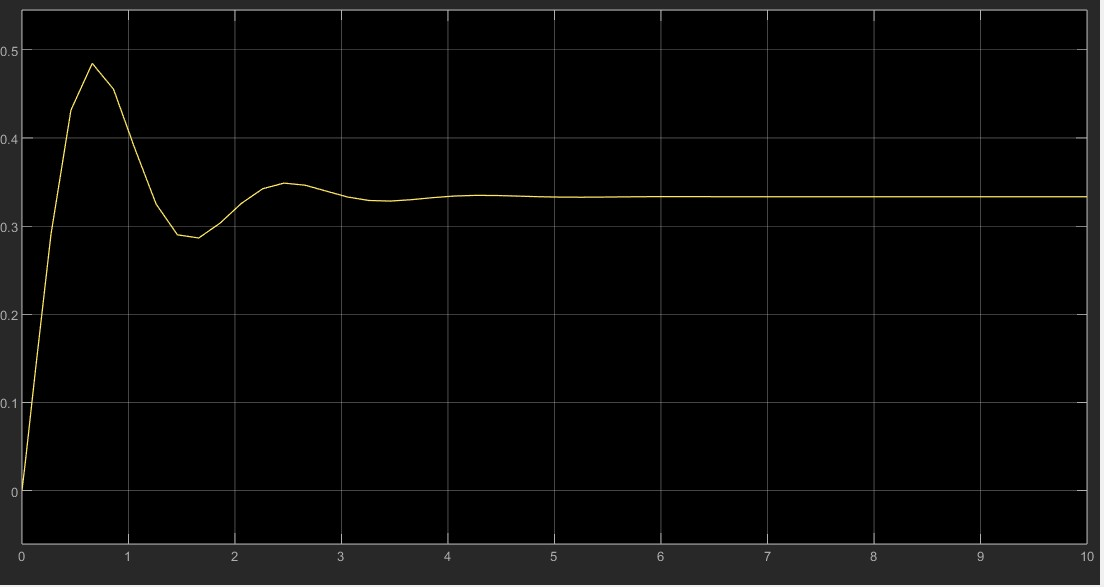
\includegraphics[scale=0.3]{canonical_controlled_form_2.jpg}
        \captionsetup{skip=0pt}
        \caption{График канонической управляемой формы}
        \label{fig:ccf2}
    \end{figure}
    \begin{figure}[H]
        \centering
        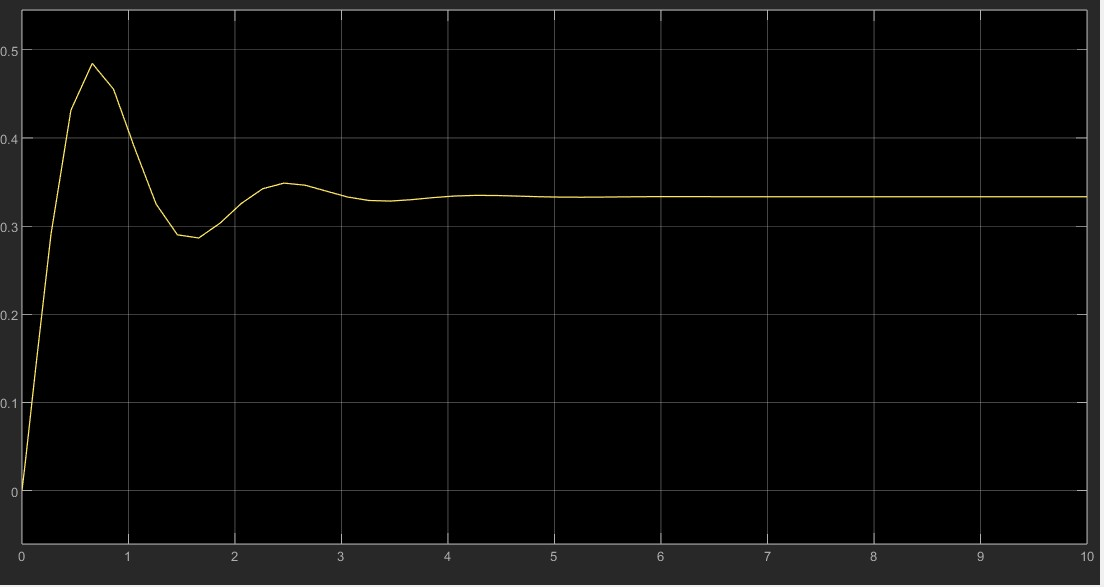
\includegraphics[scale=0.3]{canonical_observable_form_2.jpg}
        \captionsetup{skip=0pt}
        \caption{График канонической наблюдаемой формы}
        \label{fig:cof2}
    \end{figure}


    \section{Задание 3}
    \subsection{Условие}
    \textit{Замена базиса в пространстве состояний.}
    \begin{compactitem}
    \item Построить модель, подобную модели из задания 2, если матрица преобразования координат $M$ имеет вид
    $$M=\begin{bmatrix}
        2 & 0\\
        5 & 0.5
    \end{bmatrix}$$
    \item Используя блоки ``State-Space'', осуществить моделирование исходной и
    преобразованной систем при ступенчатом единичном входном воздействии и нулевых
    начальных условиях. На экран вывести выходные переменные двух систем. Схема
    моделирования представлена на рисунке \ref{fig:scheme3}
    \begin{figure}[H]
        \centering
        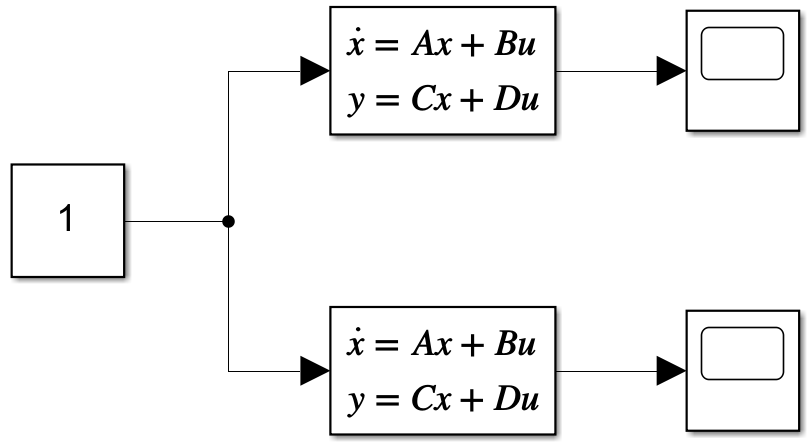
\includegraphics[scale=0.5]{scheme3.png}
        \captionsetup{skip=0pt}
        \caption{Схема эксперимента}
        \label{fig:scheme3}
    \end{figure}
    \end{compactitem}


    \subsection{Выполнение}
    Матрицы подобных моделей связаны соотношениями
    $$\hat{A}=M^{-1}AM,\ \ \hat{B}=M^{-1}B,\ \ \hat{C}=CM$$
    Проведем расчеты
    $$M^{-1}=
    \begin{bmatrix}
        2 & 0\\
        5 & 0.5
    \end{bmatrix}^{-1}=
    \begin{bmatrix}
        0.5 & 0\\
        -5 & 2
    \end{bmatrix}$$
    $$\hat{A}=M^{-1}AM=
    \begin{bmatrix}
        0.5 & 0\\
        -5 & 2
    \end{bmatrix}
    \begin{bmatrix}
        0.5 & 1\\
        -15 & -3
    \end{bmatrix}
    \begin{bmatrix}
        2 & 0\\
        5 & 0.5
    \end{bmatrix}=
    \begin{bmatrix}
        0.25 & 0.5\\
        -32.5 & -11
    \end{bmatrix}
    \begin{bmatrix}
        2 & 0\\
        5 & 0.5
    \end{bmatrix}=
    \begin{bmatrix}
        3 & 0.25\\
        -120 & -5.5
    \end{bmatrix}
    $$
    $$\hat{B}=M^{-1}B=
    \begin{bmatrix}
        0.5 & 0\\
        -5 & 2
    \end{bmatrix}
    \begin{bmatrix}
        0\\
        1
    \end{bmatrix}=
    \begin{bmatrix}
        0\\
        2
    \end{bmatrix}
    $$
    $$\hat{C}=CM=
    \begin{bmatrix}
        5 & 1
    \end{bmatrix}
    \begin{bmatrix}
        2 & 0\\
        5 & 0.5
    \end{bmatrix}=
    \begin{bmatrix}
        15 & 0.5
    \end{bmatrix}
    $$
    Передаточная функция остается такой же, как в задании 2
    $$W(p)=\dfrac{p+4.5}{p^2+2.5p+13.5}$$
    Схема моделирования представлена на рис. \ref{fig:scheme3}. Параметры в SIMULINK представлены на рис. \ref{fig:windows3}. Выведем графики.
    \begin{figure}[H]
        \centering
        \begin{subfigure}{0.3\textwidth}
            \centering
            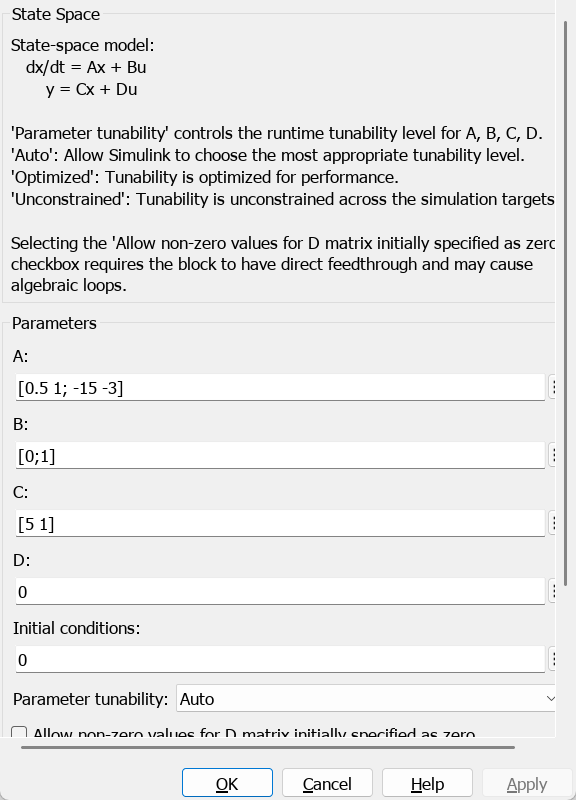
\includegraphics[width=\linewidth]{model_3_window.png}
            \caption{Параметры SIMULINK для исходной системы (см. задание 2)}
            \label{fig:m3w}
        \end{subfigure}
        \begin{subfigure}{0.3\textwidth}
            \centering
            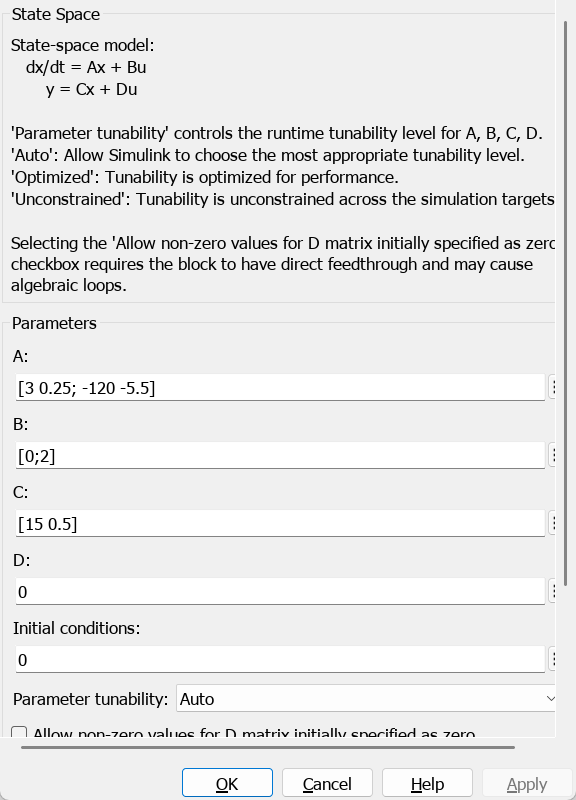
\includegraphics[width=\linewidth]{new_model_3_window.png}
            \caption{Параметры SIMULINK для преобразованной системы}
            \label{fig:nm3w}
        \end{subfigure}
        \caption{Параметры SIMULINK для ``State-Space''}
        \label{fig:windows3}
    \end{figure}
    \begin{figure}[H]
        \centering
        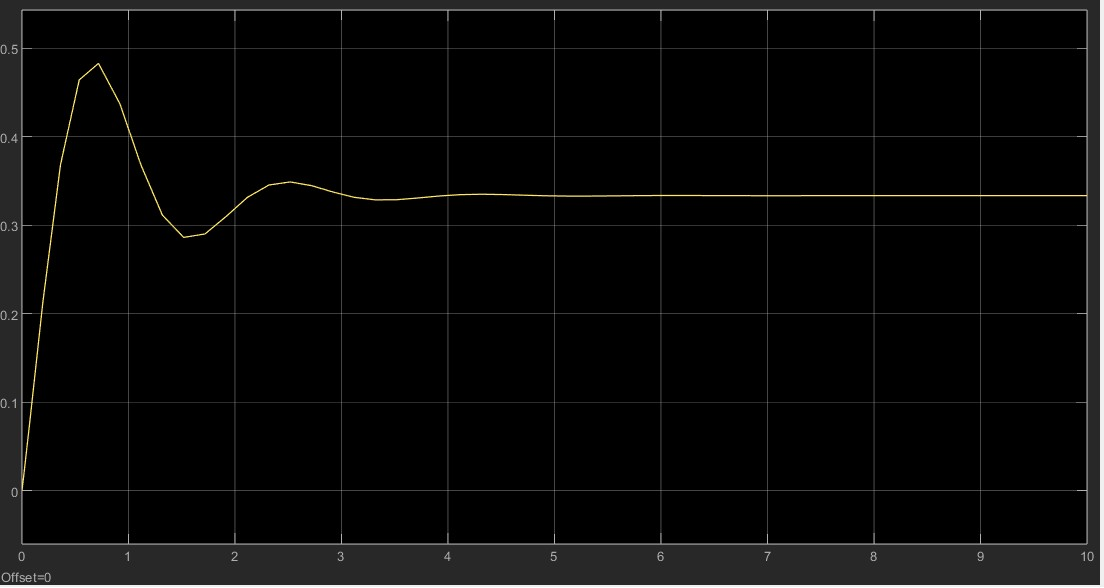
\includegraphics[scale=0.3]{model_3.jpg}
        \captionsetup{skip=0pt}
        \caption{График исходной системы}
        \label{fig:m3}
    \end{figure}
    \begin{figure}[H]
        \centering
        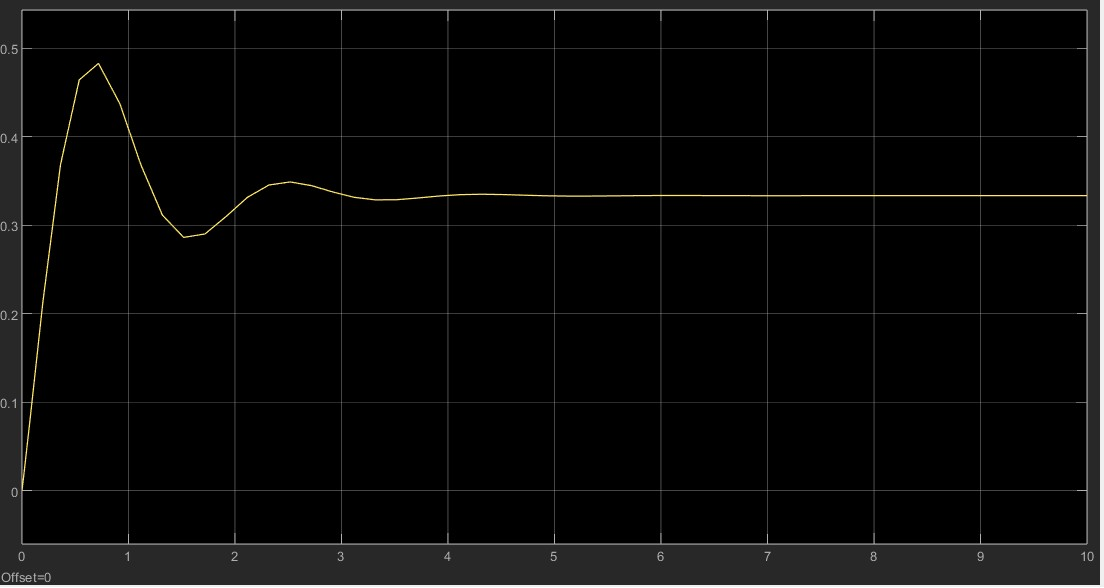
\includegraphics[scale=0.3]{new_model_3.jpg}
        \captionsetup{skip=0pt}
        \caption{График преобразованной системы}
        \label{fig:nm3}
    \end{figure}


    \section{Вывод}
    Я познакомился с методами взаимного перехода между моделями \\
    вход-выход и вход-состояние-выход, а также с каноническими формами представления
    моделей вход-состояние-выход.
    
    
    Использование канонических форм существенно упрощает решение многих практических задач,
    связанных с анализом и синтезом систем управления.
\end{document}